\chapter{Analyse de la méthode JFNK dans CEDRE}

  \paragraph{}
  In a previous chapter, we identified some methods from the literature that we wanted to use in our solver CEDRE, and some other from CEDRE we wanted to improve.
  In another chapter, we discussed the practical implementation of said methods in the solver.
  The goal of this chapter is now to test those methods on several applications to comment on the choices we made.
  We need to define test cases that represent well enough target applications so we can comment the performances of our choices.


  \section{Comparaison entre la matrice jacobienne explicite et la formulation sans matrice}

    \paragraph{}
    From our analysis and implementation, the main addition to the solver is the Jacobian Free Newton--Krylov method, and in particular the matrix-free approach.
    In this part we will then compare two methods: the traditional method and the new one that uses the matrix-free approach.
    As we are interested in implicit time integration, we will use the implicit Euler method, for reasons previously discussed.
    The traditional method linearises the equation that the implicit Euler method produces, approximates the Jacobian matrix using the Jacobian matrix of the corresponding first order scheme, and then solves the linear system with the Krylov subspace method GMRES.
    As we want to understand the impact of a better Jacobian matrix, we are only going to change how it is computed.
    The new method will then work in a similar way, except the matrix used in the linear solver is not actually computed, but the matrix-vector produces are approximated using equation (\ref{eq:matrix_free}).


    \subsection{Turbulent transonic airfoil}

      \subsubsection{Definition of the test case}


        \PS{TODO: sûr de aoa et Re ?}

        \paragraph{}
        Our first application is a typical aerodynamics test case.
        It is a 2D simulation of the flow around a RAE 2822 wing profile.
        The only fluid is standard air.
        The Mach number is taken equal to 0.75, the chord is equal to $1\si{\meter}$, the angle of attack is $2.8\si{\degree}$ and we use the atmospheric conditions at 10km.
        This gives a Reynolds number of \num{6.3e6}.

        \paragraph{}
        We decided to use this first test case for multiple reasons.
        Firstly, it is a simple case in the field of computational fluid dynamics.
        Is is a standard aerodynamics case, with a small mesh in comparaison to many other 3D cases.
        This allows us to test out methods inexpensively.
        Secondly, this case belong to the tutorial suite of our solver.
        It means that it is already well mastered by the team.
        Thirdly, even if it is only a standard aerodynamics case it still have some stiff features, such as turbulence and a shock.
        Finally, it is a standard test case for turbulence modeling validation.
        Therefore there are many references in the literature using this case. \PS{LES DONNER !}
        Even if this thesis aims at multiphysics, it is often good to start slow, and that is why we are doing with this test case.

        \paragraph{}
        The mesh used for this simulation is an unstructured hybrid mesh made of triangles and quadrangles \PS{c'est bien ça ?}.
        Parts of it can be seen on figure \ref{fig:rae_mesh}.
        Cell sizes range from $2.5\si{\meter}$ far from the airfoil and $100\si{\micro\meter}$ at the wall.
        At the wall there is a C-shaped layer of regular cells.
        This helps better capture boundary layer effects near the profile and the \PS{pas vraiment lâcher tourbillonnaire}.
        Also, at those conditions a shock is expected to develop on the upper part \PS{extrados ?}.
        Special treatment such as refinement was applied to the mesh at the expected shock location.

        \begin{figure}
          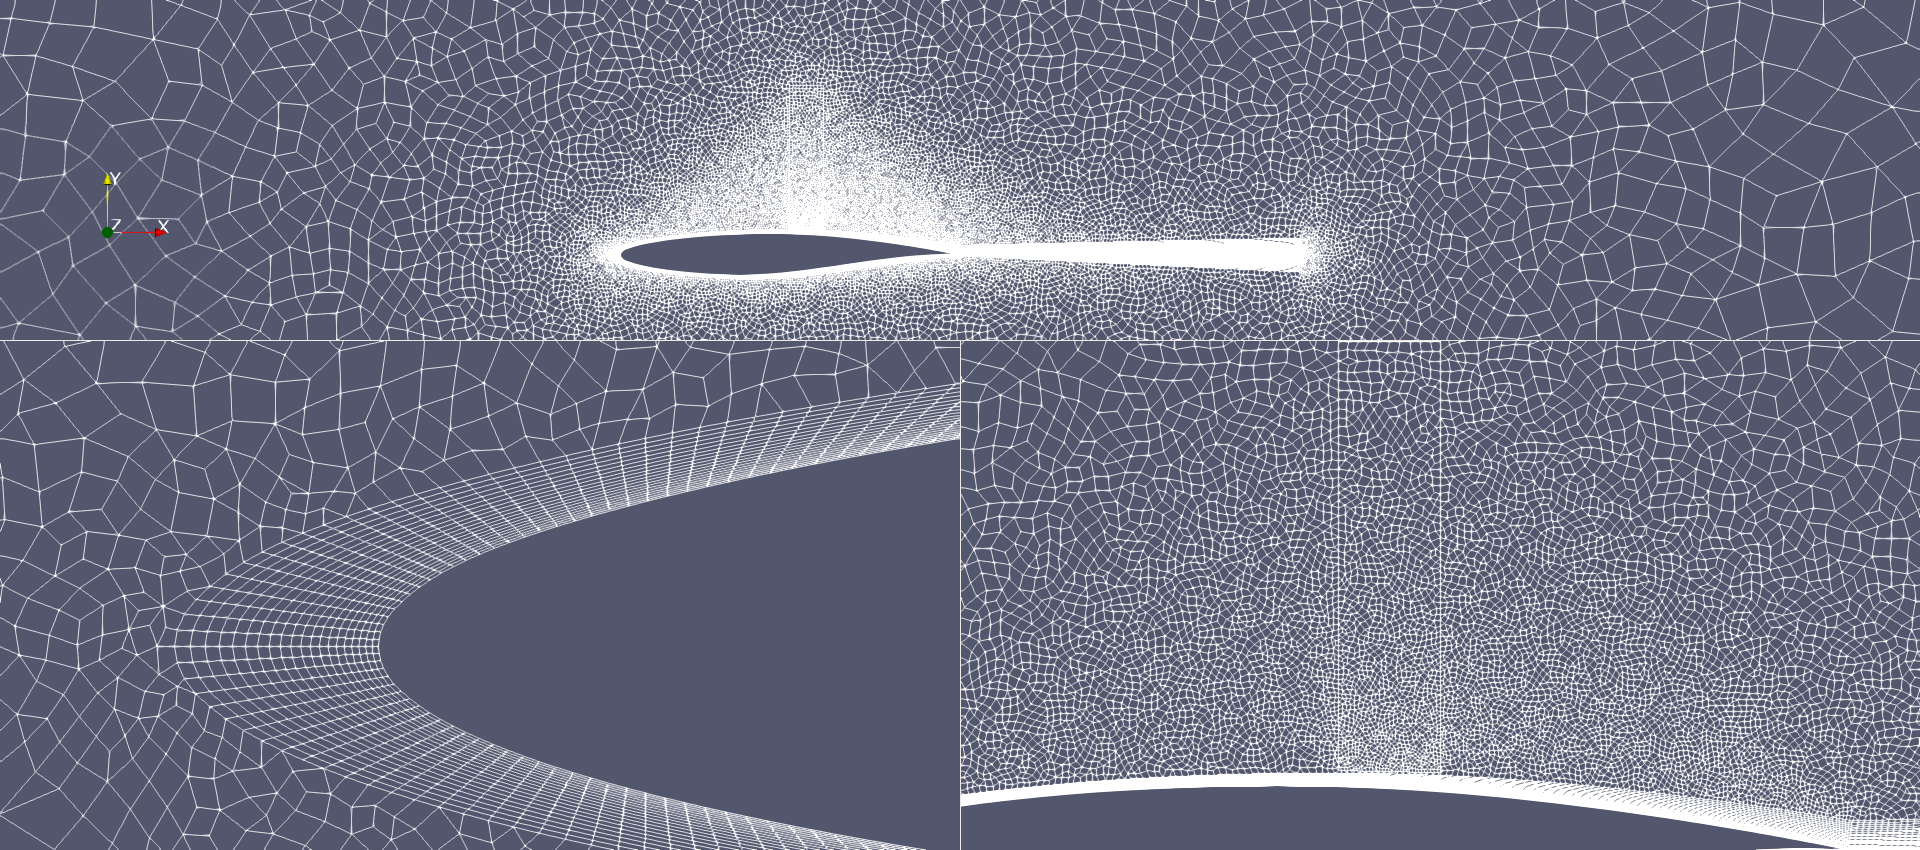
\includegraphics[width=\textwidth]{figures/rae_mesh.png}
          \caption{\PS{TODO}}
          \label{fig:rae_mesh}
        \end{figure}

        \paragraph{}
        The model used is the Reynolds Averaged Navier--Stokes equations, or RANS.
        Simply put, every scale of the turbulence is modelised \PS{c'est bien ça ?}.
        For this case, we decided to use the famous Spalart--Allmaras turbulence model.
        It is well known for being one of the simplest turbulence model, which is fine for us as we want to set up a simple first test case.

        \paragraph{}
        \PS{KEX ou MTP ? Finir introduction du cas.}


      \subsubsection{Analysis of the results}


        \paragraph{}
        Haha




    \subsection{Sphère hypersonique}


  \section{Utilisation de la formulation sans matrice sur un nouveau modèle de fluide}
    \subsection{Modèle Multi-températures}
    \subsection{Sphère hypersonique}
      \subsubsection{Modèle réactif complet}
      \subsubsection{Modèle réactif simplifié}
